\chapter{Introduction} \label{chap:intro}

\section*{Context} \label{sec:context} 
% with * not numerate the title

Consciousness is the individual's ability to be aware of the knowledge of self and the environment. Furthermore, the ability to respond to various voluntary internal and
external stimuli \citet{https://doi.org/10.1196/annals.1440.013}.
In basic neurological terms, it is composed of awareness and wakefulness \citet{zheng2017disentangling}.
The different states of consciousness are represented in the table
\ref{tab:my-table}.

\begin{table}[!htb].
\begin{tabular}{lccll}
\cline{3-3}
\multicolumn{1}{c}{{Condition}}             & \multicolumn{1}{l|}{\textbf{Wakefulness}} & \multicolumn{1}{l|}{\textbf{Awareness}} &  &  \\ \cline{3-3}
Coma                                            & -                                         & -                                       &  &  \\ \cline{1-3}
\multicolumn{1}{|l|}{Vegetative State}          & \multicolumn{1}{c|}{+ to ++}              & \multicolumn{1}{c|}{-}                  &  &  \\ \cline{1-3}
\multicolumn{1}{|l|}{Minimally Conscious State} & \multicolumn{1}{c|}{+ to ++}              & \multicolumn{1}{c|}{+}                  &  &  \\ \cline{1-3}
Emerged from Minimally Conscious State          & ++                                        & ++                                      &  & 
\end{tabular}
\caption{Disorders of consciousness categorization}
\label{tab:my-table}
\end{table}
\vspace{0.2cm}
Brain Injury (BI)  is head injury that damage in the brain and his complex connections. 

This causes
problems with how a person can
think and interact with the world around
him or her. Following a brain injury, there are
specific cognitive skills that are no
longer functioning in the same capacity.
Perception, observation and
recognition of information are deeply affected.

There are events that damage areas of the brain that control parts of the human body. And the patient's faculties are conditioned.
The origin of brain injuries can be: 
\begin{itemize}
    \item acute: as in a virus or hemorrhage  \item traumatic: like road accidents, impacts where there are head injuries  \item non-traumatic: such as drowning, sudden attacks on organs and consumption of substances harmful to the body
\end{itemize} 
That cause brain damage that leads to consequences in terms of disturbing the person's consciousness\cite{teixeira2020disorders}.

After coma, the rates of diagnostic errors, namely in the distinction between vegetative state (VS) and the minimally conscious state (MCS), are high  $\approx 40$ \cite{andrews1996misdiagnosis}  \cite{ gill2004sensory} \cite{schnakers2009diagnostic}. 

The diagnosis of the condition of the patient who suffers brain damage is made using scales to assess the behavioural response to stimulation:
CRS-r, SMART, WHIM, WNSSP, Rancho levels physicians etc. \label{behscales}
With technological advancement and the spread of its use, neuronal imaging technologies such as:
   functional magnetic resonance imaging (fMRI),
   electroencephalogram (EEG)
   positron emission tomography (PET).

  It has been possible to leverage the discovery and knowledge in the area of neuroscience and the identification, consequent diagnosis of the cerebral behavior of patients. This helps a lot in studying %\doc
  DOC because it demonstrates the level of responsiveness that could not be obtained by the behavior scales already mentioned. \ref{behscales}
  
  VS is defined as the absence of self-awareness and the environment. Behaviours are limited to reflexive activities indicating no purposeful movement, neither experience of suffering or evidence of comprehension \citet{multi1994medical}
  
  %\Mcs
  MCS is serious but does not represent a complete lack of awareness resulting  from widespread damage to the telencephalon (the part of the brain that controls thinking and behavior).
  The intentionally and types of behavior exhibited by people in a VS and a MCS,
 can be challenging to distinguish, and subtle signs of consciousness can go unnoticed.
It is widely recognized that the use of standardized and sensitive behavioral assessment scales
such as the Sensory Modality Assessment and Rehabilitation Technique (SMART), can
help healthcare professionals identify subtle signs of awareness.



\section{SMART} \label{sec:smart}

SMART is an assessment tool that combines communication, motor and sensory modalities to diagnose patients who have suffered severe brain injuries \citep{DaConceicaoTeixeira2018}.

Five levels: no response, reflex response, withdrawal response, localized response and differentiated response

Advantage:

This method is entirely credible and accepted by the healthcare community that deals with this clinical population.


Disadvantage:


It requires and consumes many resources in making the diagnosis.

\section{Diagnostic tools} \label{Diagnostic}

Neuroscientific technologies, experimental methods study the patients' brain processes through many devices, in specific: 

Neuroimaging, psychophysical techniques or psychological tests are used to study processes such as learning, attention, memory, or emotion \cite{Corchs2019}.
\espaco

The following stand out:

 
\begin{itemize}


\item Electroencephalogram (EEG)

Electroencephalography is a simple, non-invasive technique based on the recording and evaluating brain activity using electrodes placed on the skull surface. The (EEG) is the record that results from the measurement of the electrical potentials of the brain. EEG shows the electrical fluctuation in the different locations of the cortex \cite{Bender2015}. However it has the disadvantage of having an insufficient resolution to register the neuronal activity in deeper brain structures, such as the \textit{nucleus accumbens} related to the processing of emotions\cite{Lang2010}. %\citep{8701676}. 

Study using MMN tomography technique resulting in classification of patients with DOC in figure \ref{ferramentaMMN}
\begin{figure}[h!]
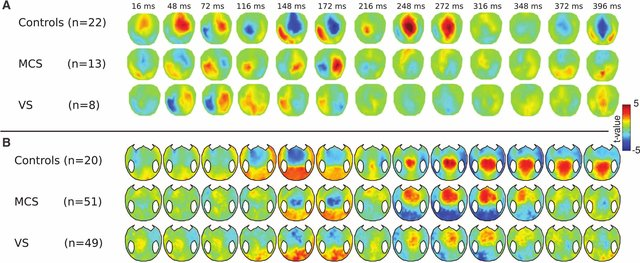
\includegraphics[scale=0.7]{figures/MMN-topography-in-patients-with-disorders-of-consciousness-and-in-healthy-controls-The_W640.jpg}
\caption[MMN topography in patients with disorders of consciousness and in healthy controls. The figure shows a comparison of (A) t test maps from Boly et al. (1) for the MMN (comparison of deviant and standard trials) with (B) similar maps obtained from 120 recordings collected in the past three years in Lionel Naccache's laboratory, Hôpital de la Salpêtrière, Paris]{MMN topography in patients with disorders of consciousness and in healthy controls \cite{King2011}
\cite{Boly2011}} %legenda imagem no indice e no texto
\label{ferramentaMMN}
\end{figure}

\item  (Functional) Magnetic Resonance

 It is a method of diagnosis and fundamental research in Market research Analyzing emotions Planning surgery Brain mapping neurosciences.\citep{fmri} It allows the analysis of the subjects' response to different activities or stimuli. Magnetic resonance imaging is a non-invasive technique used to obtain information about the subjects' response to different stimuli (very common in research and analysis of neurological diseases such as Alzheimer's Disease and also for soft tissue injuries and inflammation). This technique evaluates the activation and the emotional state of the subject when exposed to certain stimuli. \cite{noauthor_fmri_nodate}
 
 
\item  GSR (galvanic skin response)

Measurement of the galvanic response is done by placing
electrodes on the fingers. Studies measure resistance
skin and its conductance.

A GSR amplifier applies constant tension to the skin,
of such a low voltage that the individual cannot
perceive it through electrodes. The current generated in the
skin by tension can be detected and recorded. The output of the GSR amplifier determines the conductance.
The conductance of the skin gives feedback on the body's response to the stimulus, it is widely used in post-coma and coma phases
\cite{Altntop2021,Luaute2018}.



\item  Eye-tracking

 Eye-tracking refers to recording the movements of an individual's eye while examining a visual stimulus. In broad, it is responsible for measuring eye movements using a camera that quantifies them. Modern eye trackers record eye position and movement using contrast to locate the central point of the pupil and create a reflection of the cornea using infrared light. It is possible to perform the analysis of the position of the gaze and the movement of the eyes in three-dimensional environments.
Eye-tracking techniques apply to domains where interaction and interests matter,
looking to sell or immerse to improve the customer or user experience. In medicine, it is essential to recognize behaviours and patterns to investigate further and be able to characterize\cite{Ting2014}.


\item  Face reading

 Facial expressions are one of the most robust  visual methods for conveying emotions. The face plays a crucial role in the cognitive processes of individuals since the signs that show facial expressions denote internal states or emotions. The analysis of facial expressions provides valuable information when combined with other tools that allow sensory information collection, such as eye-tracking or EEG .

\end{itemize}


\espaco




Research continues on clinical tools such as (fMRI) with improved diagnostic certainty and prognostic applications. There are 3 main factors that influence the prognosis of patients in the Vegetative State (VS) and the patient's minimum state of consciousness (MCS):
\begin{itemize}
\item 
\end{itemize}
Time (the longer you stay in the state, the more complicated functional recovery becomes)
\begin{itemize}
\item 
\end{itemize}
\begin{itemize}
\item Age (young people have a higher recovery rate, linked to physiological recovery processes and brain plasticity)
\item Type (if non-traumatic, there is a shorter potential recovery window)
\item Note: The more severe the degree of injury, the rarer the recovery.
\end{itemize}


\section{Objectives} \label{sec:objectives}
With the new discoveries in the fields of technology: more properly artificial intelligence combined with machine learning, we hope to help and give a more accurate diagnosis.
\begin{enumerate}
    \item Classification in 2 possible stages (minimal state of consciousness and vegetative state)
    \item Reduce time procedures diagnosis: after the first complete goal check, reduce the number of sessions to less than 10
    \item Try to find correlations between origin and possible stages and gauge the accuracy of results with basis on number of sessions available
\end{enumerate}
\espaco



\section{Summary} \label{sec:struct}

Lorem ipsum dolor sit amet, consectetur adipiscing elit.
Mauris sem risus tempus a elit Chapter~\ref{chap:sota}.
Proin in mauris varius, auctor eros eu, accumsan est.
Suspendisse molestie elit in lacinia iaculis Chapter~\ref{chap:chap3}.
Sed lobortis sem non metus pharetra efficitur. Mauris tortor arcu,
pulvinar sit, molestie vitae libero %Chapter~\ref{chap:chap4}.
In odio felis, consectetur vel rhoncus et, iaculis et nisi.
Suspendisse rutrum felis magna Chapter~\ref{chap:concl}.


\textbf{Areas: }\\ CCS \textrightarrow   Computing \hspace{0.1cm} methodologies \textrightarrow  Machine\hspace{0.1cm} learning \\ CCS \textrightarrow   Applied \hspace{0.1cm}computing \textrightarrow    Life\hspace{0.1cm} and \hspace{0.1cm}medical \hspace{0.1cm}sciences

 